%\documentclass[portrait,final,a0paper,fontscale=0.292]{baposter}
\documentclass[portrait,a0paper,fontscale=0.31]{baposter}

\usepackage{calc}
\usepackage{graphicx}
\usepackage{amsmath}
\usepackage{amssymb}
\usepackage{relsize}
\usepackage{multirow}
\usepackage{rotating}
\usepackage{bm}
\usepackage{url}

% Redmar
\usepackage{enumitem}       %set indent for enumerate/itemize
\setitemize{leftmargin=0.3cm,itemsep=1.3em,parsep=0pt}%,topsep=0pt}
\usepackage[none]{hyphenat} %disables all hyphenation
%https://tex.stackexchange.com/questions/79591/superscripts-in-bibliography-with-bibtex
\usepackage[super]{natbib} 
\usepackage[font=small,labelfont=bf]{caption}
\DeclareCaptionFont{tiny}{\tiny}
%\usepackage{svg}
\usepackage{verbatim}

\usepackage{graphicx}
\usepackage{multicol}

%\usepackage{times}
%\usepackage{helvet}
%\usepackage{bookman}
\usepackage{palatino}

% Disable due to conflict with usepackage caption
%\newcommand{\captionfont}{\footnotesize}

\graphicspath{{images/}{../images/}}
\usetikzlibrary{calc}

%% Some names etc
\newcommand{\senterica}{\textit{Salmonella enterica} serovar Heidelberg }
\newcommand{\heidelberg}{\textit{S.} Heidelberg }
\newcommand{\fcite}[2]{#1$^#2$}
\newcommand{\mdr}{multidrug-resistant }
\newcommand{\Mdr}{Multidrug-resistant }
\newcommand{\reference}{reference strain SL476 }
\newcommand{\amr}[2]{\textbf{#1} #2,}
\newcommand{\famr}[2]{\textbf{#1} #2.}
\newcommand{\cmy}{\textit{bla}{\tiny CMY-2}}
\newcommand{\padd}{\vspace*{0.2cm}}
\newcommand{\ppadd}{\vspace*{0.29cm}}

%%%%%%%%%%%%%%%%%%%%%%%%%%%%%%%%%%%%%%%%%%%%%%%%%%%%%%%%%%%%%%%%%%%%%%%%%%%%%%
%%% Begin of Document
%%%%%%%%%%%%%%%%%%%%%%%%%%%%%%%%%%%%%%%%%%%%%%%%%%%%%%%%%%%%%%%%%%%%%%%%%%%%%%

\begin{document}

%%%%%%%%%%%%%%%%%%%%%%%%%%%%%%%%%%%%%%%%%%%%%%%%%%%%%%%%%%%%%%%%%%%%%%%%%%%%%%
%%% Here starts the poster
%%%---------------------------------------------------------------------------
%%% Format it to your taste with the options
%%%%%%%%%%%%%%%%%%%%%%%%%%%%%%%%%%%%%%%%%%%%%%%%%%%%%%%%%%%%%%%%%%%%%%%%%%%%%%
% Define some colors

%\definecolor{lightblue}{cmyk}{0.83,0.24,0,0.12}
\definecolor{lightblue}{rgb}{0.145,0.6666,1}
\definecolor{darkblue}{rgb}{.082352,.2588235,.450980}

%\hyphenation{resolution occlusions}
%%
\begin{poster}%
  % Poster Options
  {
  % Show grid to help with alignment
  grid=false,
  % Column spacing
  colspacing=2em,
  % Color style
  bgColorOne=white,
  bgColorTwo=white,
  %borderColor=lightblue,
  borderColor=white,
  headerColorOne=darkblue,
  headerColorTwo=darkblue,
  headerFontColor=white,
  boxColorOne=white,
  boxColorTwo=darkblue,
  % Format of textbox
  textborder=faded,
  % Format of text header
  eyecatcher=true,
  headerborder=closed,
  headerheight=0.1\textheight,
%  textfont=\sc, An example of changing the text font
  headershape=rounded,
  headershade=shadelr,
  headerborder=open,
  headerfont=\Large\sf\bf, %Sans Serif
  headerheight=0.13\textheight,
  textfont={\setlength{\parindent}{1.5em}},
  boxshade=plain,
%  background=shade-tb,
  background=plain,
  linewidth=2pt,
  }
  % Eye Catcher
  %{\includegraphics[height=5em]{images/nvwa.png}} 
  {}
  % Title
  {
    {
      Closely related \mdr \senterica isolates from imported poultry meat in the Netherlands
    }
    %\vspace{0.3em}
  }
  % Authors
  {
    %\vspace{0.15em}
    {\fcite{R.R. van den Berg}{1}, \fcite{S. Dissel}{1}, \fcite{C.C. van der Weijden}{1}, \fcite{M.L.B.A. Rapallini}{1}, \fcite{R. Heymans}{1}\\{\smaller $^1$ \textit{Netherlands Food and Consumer Product Safety Authority} }}
    %\vspace{0.15em}
  }
  %{Netherlands Food and Consumer Product Safety Authority}
  % University logo
  %{\includegraphics[height=10.5em]{images/rijksoverheid3.png}} 
  %{\includegraphics[height=9.5em]{images/rijksoverheid3.png}} 
  {\parbox[top][12em][t]{5em}{
\includegraphics[height=9.5em]{images/rijksoverheid4.png}}} 

%%%%%%%%%%%%%%%%%%%%%%%%%%%%%%%%%%%%%%%%%%%%%%%%%%%%%%%%%%%%%%%%%%%%%%%%%%%%%%
%%% Now define the boxes that make up the poster
%%%---------------------------------------------------------------------------
%%% Each box has a name and can be placed absolutely or relatively.
%%% The only inconvenience is that you can only specify a relative position 
%%% towards an already declared box. So if you have a box attached to the 
%%% bottom, one to the top and a third one which should be in between, you 
%%% have to specify the top and bottom boxes before you specify the middle 
%%% box.
%%%%%%%%%%%%%%%%%%%%%%%%%%%%%%%%%%%%%%%%%%%%%%%%%%%%%%%%%%%%%%%%%%%%%%%%%%%%%%
    % % A coloured circle useful as a bullet with an adjustably strong filling
    %\newcommand{\colouredcircle}{%
    %  \tikz{\useasboundingbox (-0.2em,-0.32em) rectangle(0.2em,0.32em); \draw[draw=black,fill=lightblue,line width=0.03em] (0,0) circle(0.18em);}}

%%%%%%%%%%%%%%%%%%%%%%%%%%%%%%%%%%%%%%%%%%%%%%%%%%%%%%%%%%%%%%%%%%%%%%%%%%%%%%
  \headerbox{Objective}{name=objective,column=0,row=0}{
%%%%%%%%%%%%%%%%%%%%%%%%%%%%%%%%%%%%%%%%%%%%%%%%%%%%%%%%%%%%%%%%%%%%%%%%%%%%%%
    \ppadd
    \noindent To examine the diversity of \mdr \senterica isolates in poultry meat imported from South America. 
 }


%%%%%%%%%%%%%%%%%%%%%%%%%%%%%%%%%%%%%%%%%%%%%%%%%%%%%%%%%%%%%%%%%%%%%%%%%%%%%%
  %\headerbox{Introduction}{name=introduction,column=0,row=1} {
  \headerbox{Introduction}{name=introduction,below=objective} {
    \padd
    \begin{itemize}
      \item Infection with \heidelberg is one of the leading causes of Salmonellosis in North America.
      \item \Mdr \heidelberg isolates were identified in poultry meat imported from South America into the Netherlands.
      \item Whole Genome Sequencing (WGS) was used to investigate this potential public health risk.
    \end{itemize}
  }
  \headerbox{Materials and Methods}{name=MM,below=introduction} {
    \padd
    \begin{itemize}
      \item A retrospective study was performed to investigate the diversity of isolates from Brazil (n=114) and Argentina (n=2) isolated between 2010 and 2014.
      \item Isolates were sequenced using Illumina HiSeq 2500. As controls, two independent poultry batches were sampled and sequenced five times, and a single isolate was sequenced twice.
      \item Isolates were tested for antimicrobial susceptibility (Sensititre) and the presence of resistance genes (PCR).
      \item Publicly available Illumina reads from three separate outbreaks (n=5 per outbreak) in \fcite{Canada}{1} were included in the analysis, as were isolates from \fcite{Thailand}{2} (n=2) and \fcite{Colombia}{3} (n=2).
      \item Quality control was performed with FastQC and Trimmomatic. \!Reads were mapped against \heidelberg \reference using BWA.
      \item Single Nucleotide Polymorphisms (SNPs) with a read depth $\geq\!\!\!5$ were called based on the GATK~best practices. 
      \item Concatenated SNPs were analysed with RAxML, and bootstrap support was calculated (cut-off $\geq\!80$).
      \item Multilocus Sequence Types (MLST) were determined from the WGS data using the \textit{Salmonella enterica} scheme from pubmlst.org
    \end{itemize}
  }

%%%%%%%%%%%%%%%%%%%%%%%%%%%%%%%%%%%%%%%%%%%%%%%%%%%%%%%%%%%%%%%%%%%%%%%%%%%%%%
%%%%%%%%%%%%%%%%%%%%%%%%%%%%%%%%%%%%%%%%%%%%%%%%%%%%%%%%%%%%%%%%%%%%%%%%%%%%%%
  \headerbox{Results}{name=results,column=1,span=2} {
    \padd
    \setlength{\multicolsep}{0pt}
    \begin{multicols}{2}
      \begin{itemize}
          \item Isolates from Brazil, Argentina, Colombia, Thailand, and three separate Canadian outbreaks were all classified into separate clusters, see \textbf{Figure 1}.
          \item The control isolate that was sequenced twice clustered as expected, as did the majority of the batch control isolates.
          \item A single isolate from the batch control did not cluster, most likely because the batch contained meat from multiple sources.
          \item All isolates were characterised as Multilocus Sequence Type 15, except for one isolate which had a single SNP in the \textit{thrA-12} allele.

      \columnbreak

      \item \textbf{Table 1} shows the different antimicrobial resistance profiles (EUCAST cut-off values).

      %%%%%%%%%%%%%%%% TABLE %%%%%%%%%%%%%%%% 
      {\tiny
     \setlength\tabcolsep{3.5 pt}
     \begin{tabular}{c c c c c c c c c c | c}
       \multicolumn{10}{c}{Antibiotic resistance profiles} & \shortstack{Isolates\\(n=116)} \\
       \hline
           &     &     & CIP &     & NAL & SMX & TET &     &     &13 \\
           &     &     & CIP &     & NAL & SMX & TET & GEN &     & 5 \\
       AMP &     &     & CIP &     & NAL &     & TET &     & CHL & 1 \\
       AMP & FOT & TAZ & CIP &     & NAL &     &     &     &     & 1 \\
       AMP & FOT & TAZ &     &     &     & SMX & TET &     &     & 1 \\
       AMP & FOT &     & CIP &     & NAL & SMX & TET & GEN &     & 1 \\
       AMP & FOT & TAZ & CIP &     & NAL & SMX & TET &     &     &92 \\
       AMP & FOT & TAZ & CIP & COL & NAL & SMX & TET &     &     &2 \\
       %Total&     &     &     &     &     &     &     & 117\\
     \end{tabular}
     \captionsetup{font=tiny,labelformat=empty,margin=0.6cm}
    \captionof{table}{\amr{AMP}{Ampicillin} \amr{FOT}{Cefotaxime} \amr{TAZ}{Ceftazidime} \amr{CIP}{Ciprofloxacin} \amr{COL}{Colistin} \amr{NAL}{Nalidixic Acid} \amr{SMX}{Sulfamethoxazole}   \amr{TET}{Tetracycline} \amr{GEN}{Gentamicin} \famr{CHL}{Chloramphenicol}}
    }
    %%%%%%%%%%%%%%%% TABLE %%%%%%%%%%%%%%%% 

      \item Among the 97 cephalosporin-resistant isolates, 94 exhibited AmpC phenotype and were PCR-positive for \cmy, whereas only 3 lacked \cmy. Three isolates were not tested.
      \end{itemize}
    \end{multicols}

  \captionof{figure}{}
  \noindent{\centering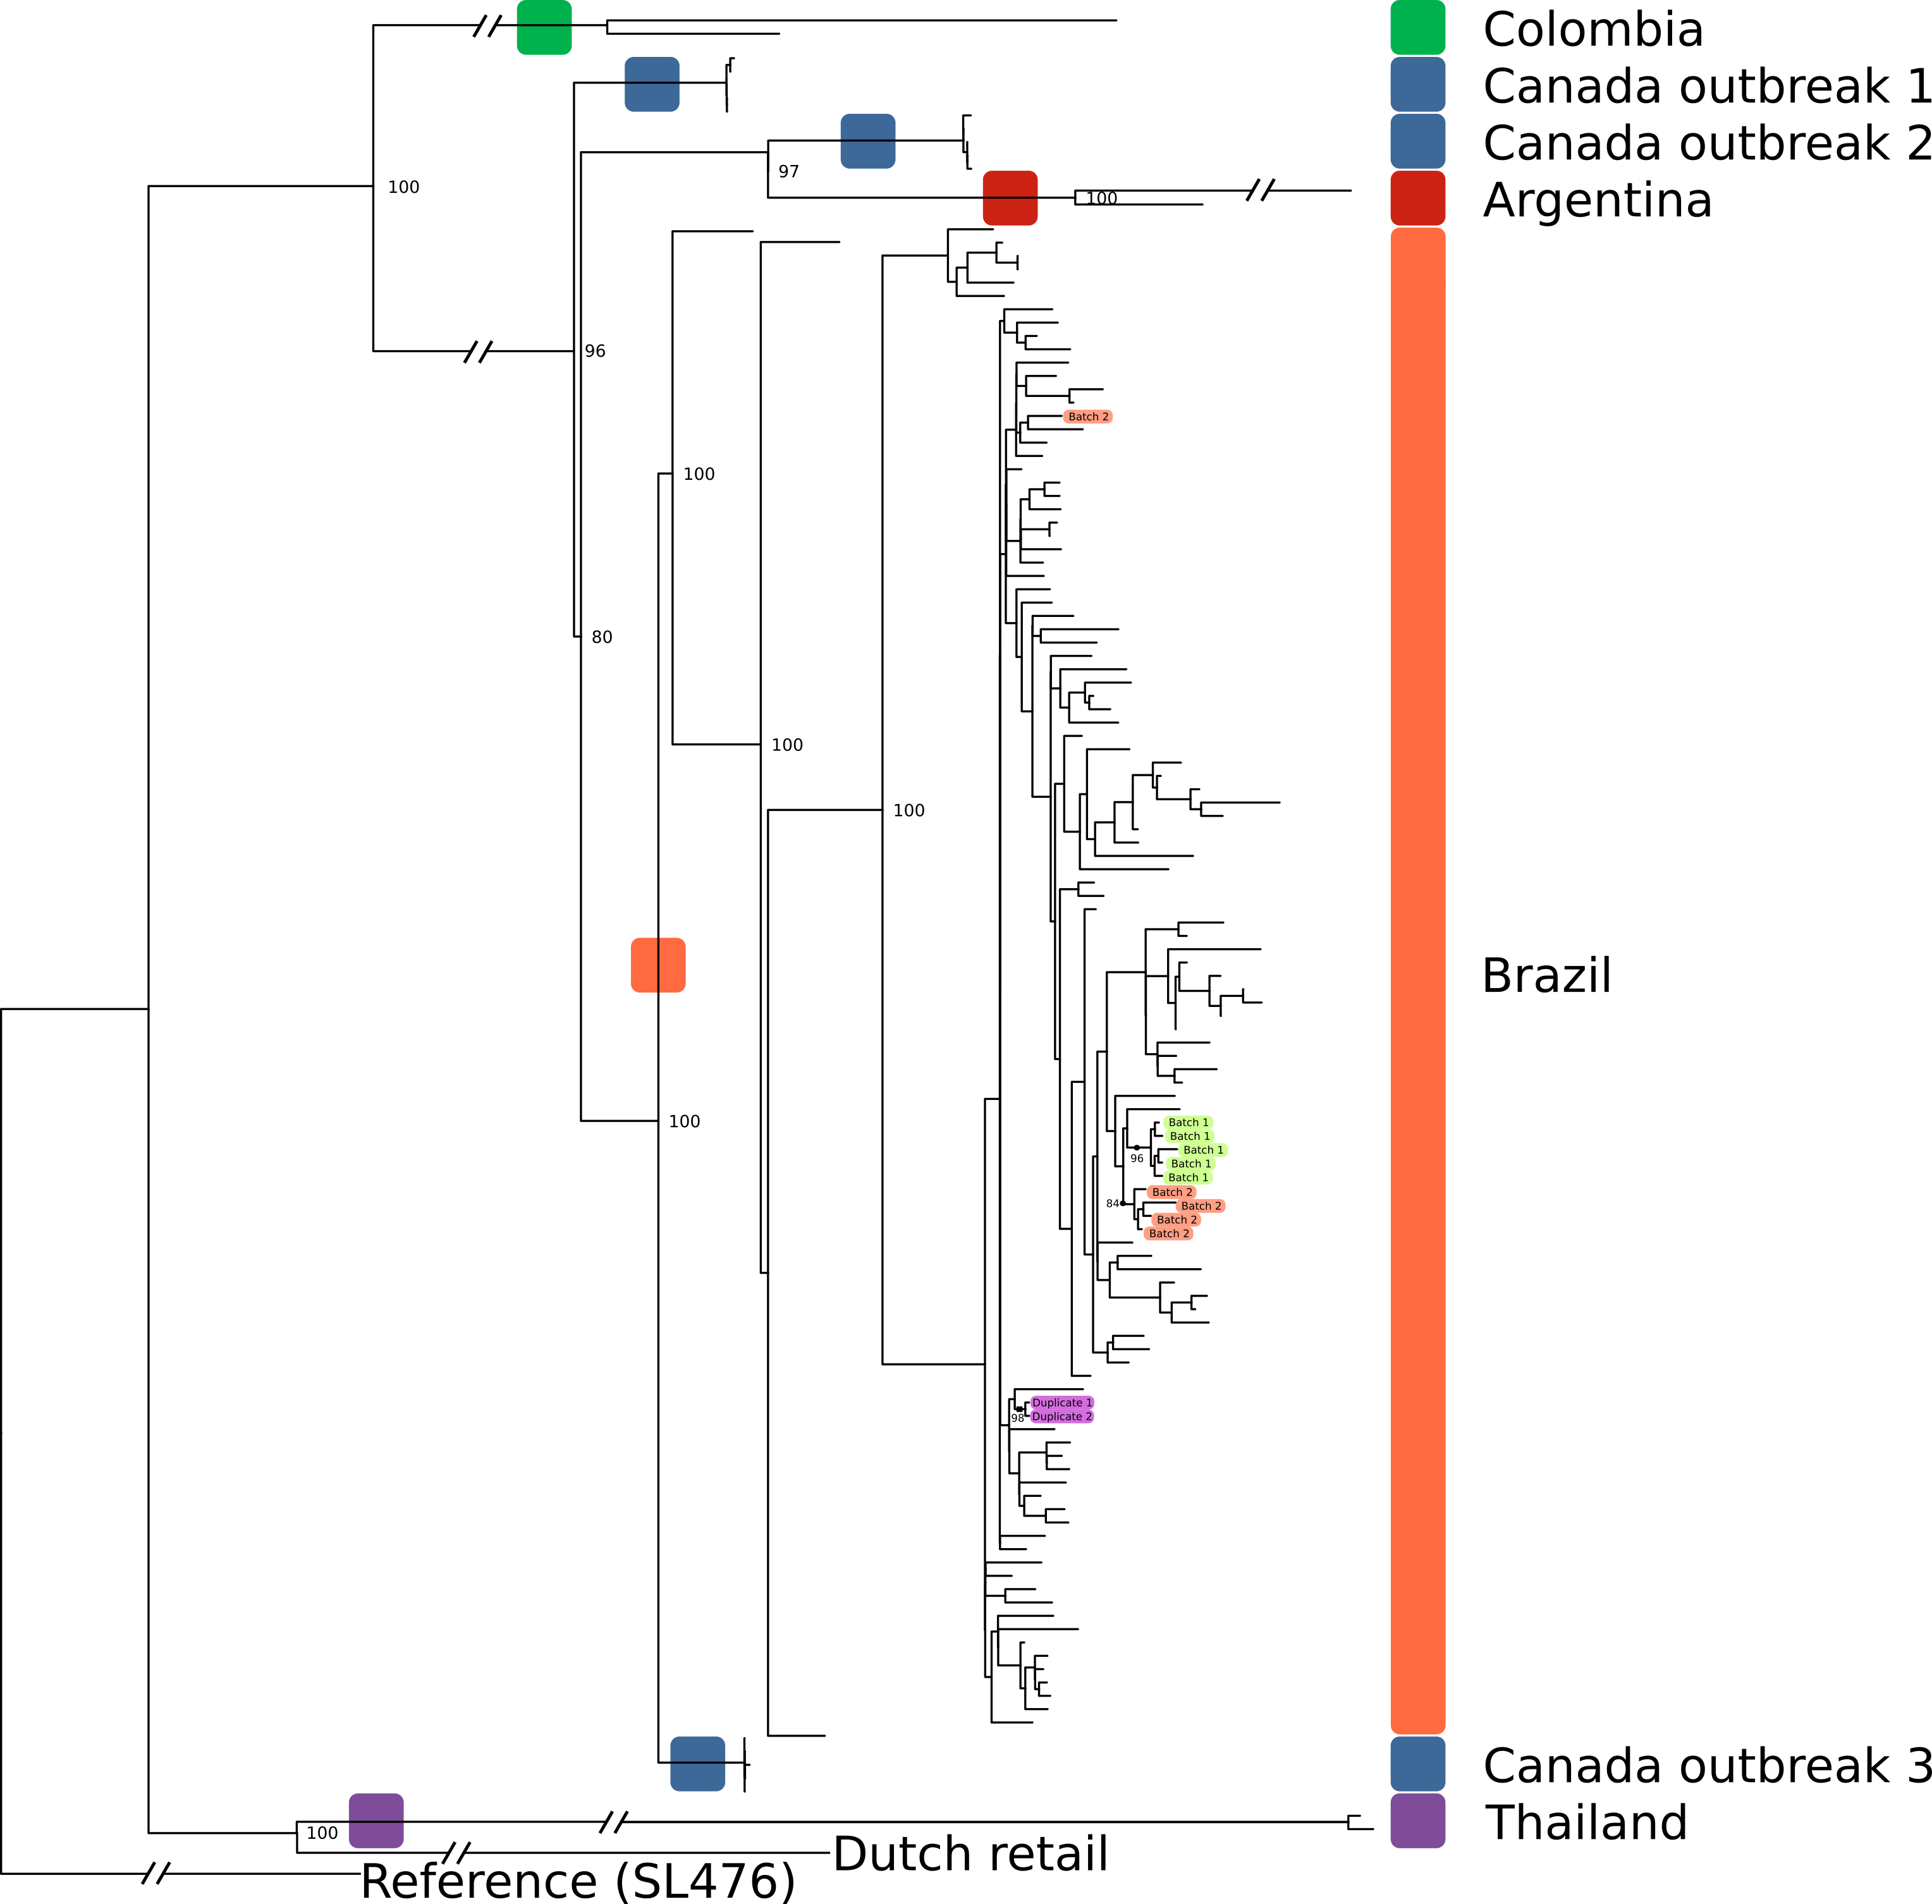
\includegraphics[width=0.75\linewidth]{images/Tree8_1.png}\\}
  \captionsetup{labelformat=empty,margin=0.6cm}
  \captionof{figure}{Maximum Likelihood clustering of isolates. Only bootstrap values $\geq\!80$ are shown.}
  %\noindent{\centering\includegraphics[width=0.75\linewidth]{../tmp/Tree3.png}\\}
  }

    %\caption{SMX: Sulfamethoxazole; CIP: Ciprofloxacin; NAL: Nalidixic Acid; TET: Tetracycline; AMP: Ampicillin; CHL: Chloramphenicol; FOT: Cefotaxime; TAZ: Ceftazidime; GEN: Gentamicin; COL: Colistin}

%%%%%%%%%%%%%%%%%%%%%%%%%%%%%%%%%%%%%%%%%%%%%%%%%%%%%%%%%%%%%%%%%%%%%%%%%%%%%%
  \headerbox{Discussion}{name=discussion,column=1,span=2,below=results} {
%%%%%%%%%%%%%%%%%%%%%%%%%%%%%%%%%%%%%%%%%%%%%%%%%%%%%%%%%%%%%%%%%%%%%%%%%%%%%%
    \padd
    \begin{multicols}{2}
    \begin{itemize}
      %\item The SNP tree successfully clusters all outbreaks, control samples, etc.
      \item While MLST assigned the same Sequence Type to each isolate, the SNP analysis can reliably differentiate isolates from different outbreaks and countries.
      \item The closely related isolates from Brazil show high diversity with few sub-clusters, which suggests that our study only captured a small subset of the existing diversity in Brazil.
      %\item This suggests a diverse, endemic population of \heidelberg that infects poultry meat from Brazil.
      \item The high diversity of \heidelberg isolates suggests the presence of an endemic, \mdr population in the poultry chain in Brazil.
      \item WGS based high-resolution surveillance provides reliable clustering of \heidelberg isolates for use in food-borne outbreaks.\newline
    \end{itemize}
    \end{multicols}
  }

%%%%%%%%%%%%%%%%%%%%%%%%%%%%%%%%%%%%%%%%%%%%%%%%%%%%%%%%%%%%%%%%%%%%%%%%%%%%%%
  \headerbox{References}{name=ref,column=2,above=bottom} {
%%%%%%%%%%%%%%%%%%%%%%%%%%%%%%%%%%%%%%%%%%%%%%%%%%%%%%%%%%%%%%%%%%%%%%%%%%%%%%
    \begin{enumerate}[itemsep=-0.3ex,leftmargin=0.29cm]
      \tiny
      \item Bekal, S., et al. "Usefulness of hqSNV analysis for subtyping the highly clonal and the most prevalent Salmonella Heidelberg clone in the context of outbreak investigations." Journal of Clinical Microbiology (2015): JCM-02200.
      \item SRA SRR1060651, SRR1060668 (https://www.ncbi.nlm.nih.gov/bioproject/203445)
      \item Donado-Godoy, Pilar, et al. "Genome Sequences of Multidrug-Resistant Salmonella enterica Serovar Paratyphi B (dT+) and Heidelberg Strains from the Colombian Poultry Chain." Genome announcements 3.5 (2015): e01265-15.
    \end{enumerate}
  }

%%%%%%%%%%%%%%%%%%%%%%%%%%%%%%%%%%%%%%%%%%%%%%%%%%%%%%%%%%%%%%%%%%%%%%%%%%%%%%
\headerbox{Contact}{name=contact,column=1, aligned=ref}
%%%%%%%%%%%%%%%%%%%%%%%%%%%%%%%%%%%%%%%%%%%%%%%%%%%%%%%%%%%%%%%%%%%%%%%%%%%%%%
  {
  \begin{center}
  \vspace{1.25em}

  \textbf{R.R.vandenBerg@nvwa.nl}\linebreak
  \textbf{R.Heijmans@nvwa.nl}\linebreak
%\linebreak\linebreak\linebreak\linebreak
  \end{center}
  }


%%%%%%%%%%%%%%%%%%%%%%%%%%%%%%%%%%%%%%%%%%%%%%%%%%%%%%%%%%%%%%%%%%%%%%%%%%%%%%
\headerbox{QR Code}{name=qr,column=0,aligned=ref}
%%%%%%%%%%%%%%%%%%%%%%%%%%%%%%%%%%%%%%%%%%%%%%%%%%%%%%%%%%%%%%%%%%%%%%%%%%%%%%
  {
  %hfill to align right: https://tex.stackexchange.com/questions/55472/how-to-make-text-aligned-left-center-right-in-the-same-line
  \vspace{-0.3em}
  \begin{center}
  %\includegraphics[width=0.25\linewidth]{images/meegid_poster2016.png}
  
\includegraphics[width=0.25\linewidth]{images/meegid_heidelberg_poultry.png}
  \end{center}
  }
\end{poster}

\end{document}

